%%% 编译:XeLaTex. 
\documentclass[a4paper,UTF8]{article}
\usepackage{ctex}
\usepackage[margin=1.25in]{geometry}
\usepackage{color}
\usepackage{graphicx}
\usepackage{amssymb}
\usepackage{amsmath}
\usepackage{float}
\usepackage{amsthm}
\usepackage{enumerate}
\usepackage{bm}
\usepackage{hyperref}
\numberwithin{equation}{section}
%\usepackage[thmmarks, amsmath, thref]{ntheorem}
\usepackage{tikz}
\usetikzlibrary{trees,shapes,arrows.meta,positioning}
\usepackage{xcolor}
\theoremstyle{definition}
\newtheorem*{solution}{解答}
\newtheorem*{prove}{Proof}
\newcommand{\indep}{\rotatebox[origin=c]{90}{$\models$}}
\usepackage{caption}
\captionsetup[table]{labelsep=space} 
\usepackage{multirow}
\usepackage{fontspec}
\usepackage{xeCJK}
\usepackage{algpseudocode}
\usepackage{algorithm}
\usepackage{listings}
\usepackage{tcolorbox}


\lstdefinestyle{github}{
    backgroundcolor=\color{white},   % 设置背景颜色
    commentstyle=\color{teal},       % 注释的颜色
    keywordstyle=\color{blue},       % 关键词的颜色
    numberstyle=\tiny\color{gray},   % 行号的颜色
    stringstyle=\color{purple},      % 字符串的颜色
    basicstyle=\ttfamily\footnotesize,
    breakatwhitespace=false,         % 在空白处自动断行
    breaklines=true,                 % 自动断行
    captionpos=b,                    % 标题位置在底部
    keepspaces=true,                 % 保持空格不变
    numbers=left,                    % 行号显示在左侧
    numbersep=10pt,                  % 行号与代码的距离
    showspaces=false,                % 显示空格(用特殊下划线)
    showstringspaces=false,          % 字符串中的空格不特殊显示
    showtabs=false,                  % 显示制表符(用特殊下划线)
    tabsize=2,                       % 制表符占用的字符数
    frame=single,                    % 添加框架
    rulecolor=\color{gray},          % 框架颜色
    framexleftmargin=5mm,            % 框架扩展到左边的距离
    xleftmargin=5mm                  % 代码整体向右移动
}


%--

%--
\begin{document}
\title{机器学习与数据挖掘- 第二次作业\\ 选取最优划分准则构造决策树}
\maketitle

\section{决策树-信息增益准则}
\begin{enumerate}[\textbf{题目 1:}] % {(}1{)}
\item 考虑下面的训练集:共计6个训练样本,每个训练样本有三个维度的特征属性和标记信息。详细信息如表1所示。

请通过训练集中的数据训练一棵决策树,要求通过“信息增益”(information gain)为准则来选择划分属性。请参考《机器学习》(周志华)书中图4.4,给出详细的计算过程并画出最终的决策树。

\begin{table}[htb]   
	\begin{center}   
		\caption{训练集信息}  
		\label{table:1} 
		\begin{tabular}{|c|c|c|c|c|} \hline   
\text{序号}  &  \text{特征 A}  & \text{特征 B}   & \text{特征 C}  &  \text{标记}  \\ \hline  
1  & 0 & 1 & 1  &0  \\ \hline
2  & 1 & 1 & 1  &0  \\ \hline
3  & 0 & 0 & 0  &0  \\ \hline
4  & 1 & 1 & 0  &1  \\ \hline
5  & 0 & 1 & 0  &1  \\ \hline
6  & 1 & 0 & 1  &1  \\ \hline
		\end{tabular}   
	\end{center}   
\end{table}
\end{enumerate}

%%%%%%%%%%%%  以下是解答  %%%%%%%%%%%%%%%%%%%%%%%%%%%%
\begin{solution}

对于当前样本集合$D$中第$k$类样本所占的比例为$p_k (k=1,2,...,|y|)$,则D的\textbf{信息熵}定义为:

\begin{equation}
Ent(D)=-\sum_{k=1}^{|y|}p_k\log_{2}{p_k}
\end{equation}

假设离散属性$a$有$V$个可能的取值$\{a^1,a^2,...,a^V\}$,使用$a$对样本集$D$进行划分,产生V个分支结点,其中第$v$个节点包含了$D$中所有在$a$上取值为$a^v$的样本,记为$D^v$。属性$a$对样本集$D$进行划分所获得的\textbf{信息增益}定义为:

\begin{equation}
Gain(D,a)=Ent(D)-\sum_{v=1}^{V}\dfrac{|D^v|}{|D|}Ent(D^v)
\end{equation}

在决策树学习开始时,根节点包含D中所有的样例,其中标记为1占比$p_1=\frac{3}{6}$,标记为0占比$p_2=\frac{3}{6}$,则根节点的信息熵为
\begin{align*}
Ent(D) &= -\sum_{k=1}^{2}p_k\log_{2}{p_k} \\
       &= -(\dfrac{3}{6}\log_{2}{\dfrac{3}{6}}+\dfrac{3}{6}\log_{2}{\dfrac{3}{6}}) \\
       &= 1
\end{align*}

然后计算属性集合{特征A,特征B,特征C}中每个属性的信息增益。
\begin{itemize}
    \item 特征A 

        使用该属性对$D$进行划分,得到2个子集,分别记为:$D^1(A=1)$,$D^2(A=0)$。划分后的2个分支的信息熵为
        \begin{align*}
            &Ent(D^1) = -(\dfrac{2}{3}\log_{2}{\dfrac{2}{3}}+\dfrac{1}{3}\log_{2}{\dfrac{1}{3}}) = 0.918 \\
            &Ent(D^2) = -(\dfrac{1}{3}\log_{2}{\dfrac{1}{3}}+\dfrac{2}{3}\log_{2}{\dfrac{2}{3}}) = 0.918
        \end{align*}

        则“特征A”的信息增益为
        \begin{align*}
            Gain(D,A) &= Ent(D)-\sum_{v=1}^{2}\dfrac{D^v}{D}Ent(D^v) \\
                      &= 1 - (\dfrac{3}{6} \times 0.918 + \dfrac{3}{6} \times 0.918) \\
                      &= 0.082
        \end{align*}
        
    \item 特征B

        使用该属性对$D$进行划分,得到2个子集,分别记为:$D^1(B=1)$,$D^2(B=0)$。划分后的2个分支的信息熵为
        \begin{align*}
            &Ent(D^1) = -(\dfrac{2}{4}\log_{2}{\dfrac{2}{4}}+\dfrac{2}{4}\log_{2}{\dfrac{2}{4}}) = 1 \\
            &Ent(D^2) = -(\dfrac{1}{2}\log_{2}{\dfrac{1}{2}}+\dfrac{1}{2}\log_{2}{\dfrac{1}{2}}) = 1
        \end{align*}

        则“特征B”的信息增益为
        \begin{align*}
            Gain(D,B) &= Ent(D)-\sum_{v=1}^{2}\dfrac{D^v}{D}Ent(D^v) \\
                      &= 1 - (\dfrac{4}{6} \times 1 + \dfrac{2}{6} \times 1) \\
                      &= 0
        \end{align*}
    
    \item 特征C
    
        使用该属性对$D$进行划分,得到2个子集,分别记为:$D^1(C=1)$,$D^2(C=0)$。划分后的2个分支的信息熵为
        \begin{align*}
            &Ent(D^1) = -(\dfrac{1}{3}\log_{2}{\dfrac{1}{3}}+\dfrac{2}{3}\log_{2}{\dfrac{2}{3}}) = 0.918 \\
            &Ent(D^2) = -(\dfrac{2}{3}\log_{2}{\dfrac{2}{3}}+\dfrac{1}{3}\log_{2}{\dfrac{1}{3}}) = 0.918
        \end{align*}

        则“特征C”的信息增益为
        \begin{align*}
            Gain(D,C) &= Ent(D)-\sum_{v=1}^{2}\dfrac{D^v}{D}Ent(D^v) \\
                      &= 1 - (\dfrac{3}{6} \times 0.918 + \dfrac{3}{6} \times 0.918) \\
                      &= 0.082
        \end{align*}
    
\end{itemize}

由此看出,$Gain(D,A)$与$Gain(D,C)$相等且最大,选取特征A作为根节点划分属性。当前划分结果如图:

\begin{figure}[H]
    \centering
    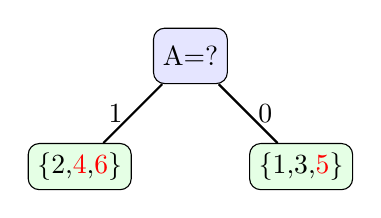
\begin{tikzpicture}
      [sibling distance=8em,
      level distance=4em,
      edge from parent/.style={draw, thick},
      edge from parent node/.style={fill=none, inner sep=1pt, draw=none},
      node style1/.style={draw, rectangle, rounded corners, align=center, minimum size=2em, fill=blue!10},
      node style2/.style={draw, rectangle, rounded corners, align=center, fill=green!10}
      ]
    
      \node[node style1] {A=?}
        child { 
            node[node style2] {\{2,\textcolor{red}{4},\textcolor{red}{6}\}} 
            edge from parent node[left] {1}
        }
        child { 
            node[node style2] {\{1,3,\textcolor{red}{5}\}}
            edge from parent node[right] {0}
        };
    \end{tikzpicture}
    \caption{}
    \label{fig:fig1}
\end{figure}

接下来,对于第一分支节点与第二个分支节点,如上进行同样计算。基于$D^1$和$D^2$分别计算出各属性的信息增益:
\begin{align*}
    Gain(D^1, B) = 0.252, \hspace{1em} Gain(D^1, C) = 0.252; \\
    Gain(D^2, B) = 0.252, \hspace{1em} Gain(D^2, C) = 0.252.
\end{align*}

对于两个分支节点,特征B与特征C分别均取得最大的信息增益。选取B作为第一个分支节点的划分属性,选取C作为第二个分支节点的划分属性。\\

由此,更新决策树:

\begin{figure}[H]
    \centering
    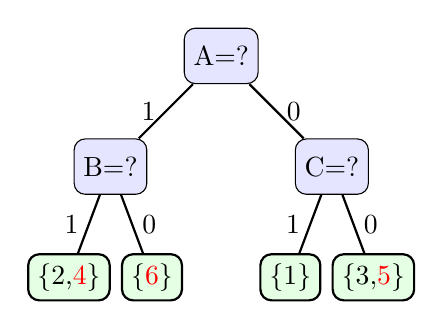
\begin{tikzpicture}
      [sibling distance=8em,
      level distance=4em,
      edge from parent/.style={draw, thick},
      edge from parent node/.style={fill=none, inner sep=1pt, draw=none},
      node style1/.style={draw, rectangle, rounded corners, align=center, minimum size=2em, fill=blue!10},
      node style2/.style={draw, rectangle, rounded corners, align=center, fill=green!10}
      ]
    
      \node[node style1] {A=?}
        child { 
            node[node style1] {B=?} [sibling distance=3em]
            child { node[node style2] {\{2,\textcolor{red}{4}\}} edge from parent node[left] {1} }
            child { node[node style2] {\{\textcolor{red}{6}\}} edge from parent node[right] {0} }
            edge from parent node[left] {1}
        }
        child { 
            node[node style1] {C=?} [sibling distance=3em]
            child { node[node style2] {\{1\}} edge from parent node[left] {1} }
            child { node[node style2] {\{3,\textcolor{red}{5}\}} edge from parent node[right] {0} }
            edge from parent node[right] {0}
        };
    \end{tikzpicture}
    \caption{}
    \label{fig:fig2}
\end{figure}


由于对B划分后的第一个节点的样例集合$D^1$和最对C划分后第二个节点的样例集合$D^2$依旧不纯,B划分后的第一个节点信息熵$Ent(D^1)=1$和C划分后的第二个节点信息熵$Ent(D^2)=1$,则经过B和C划分的节点需要分别使用特征C和B继续划分。

由B划分的第一个节点(图二\ref{fig:fig1}以B为根节点的树的左子节点)由C继续划分的信息增益为
\begin{align*}
    Gain(D^1, C) &= 1
\end{align*}

由C划分的第二个节点(图二\ref{fig:fig1}以C为根节点的树的右子节点)由B继续划分的信息增益为
\begin{align*}
    Gain(D^2, B) &= 1
\end{align*}

\vspace{8pt}

至此,得到了\textbf{最终的决策树}:

\begin{figure}[H]
    \centering
    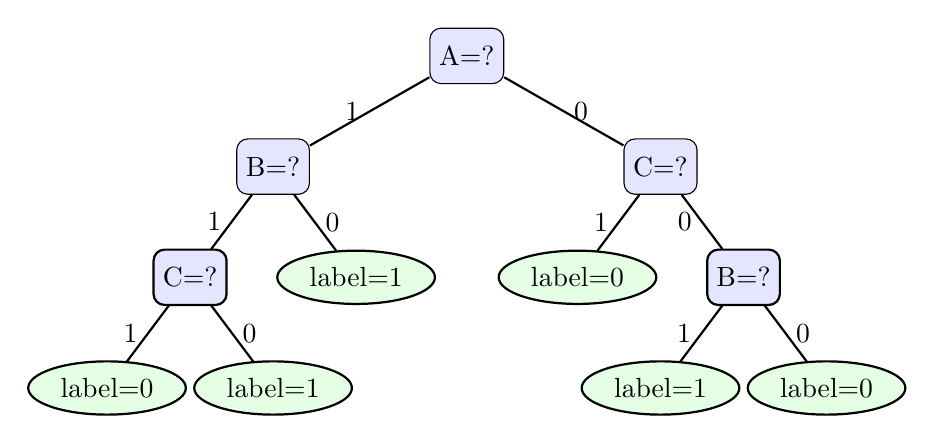
\begin{tikzpicture}
      [level distance=4em,
      node style1/.style={draw, rectangle, rounded corners, align=center, minimum size=2em, fill=blue!10},
      node style2/.style={draw, ellipse, align=center, fill=green!10, minimum width=2em, minimum height=1em},
      edge from parent/.style={draw, thick},
      edge from parent node/.style={fill=none, inner sep=1pt, draw=none},
      ]
    
      \node[node style1] {A=?} [sibling distance=14em]
        child { 
            node[node style1] {B=?} [sibling distance=6em]
            child { 
                node[node style1] {C=?} [sibling distance=6em]
                child { node[node style2] {label=0} edge from parent node[left] {1} }
                child { node[node style2] {label=1} edge from parent node[right] {0} }
                edge from parent node[left] {1} }
            child { node[node style2] {label=1} edge from parent node[right] {0} }
            edge from parent node[left] {1}
        }
        child { 
            node[node style1] {C=?} [sibling distance=6em]
            child { node[node style2] {label=0} edge from parent node[left] {1} }
            child { 
                node[node style1] {B=?} [sibling distance=6em]
                child { node[node style2] {label=1} edge from parent node[left] {1} }
                child { node[node style2] {label=0} edge from parent node[right] {0} }
                edge from parent node[left] {0} }
            edge from parent node[right] {0}
        };
    \end{tikzpicture}
    \caption{}
    \label{fig:fig2}
\end{figure}

\end{solution}

\bigskip

\begin{enumerate}[\textbf{题目 2:}] % {(}1{)}
\item 模仿给出算法ID3的程序,实现算法C4.5在西瓜数据集2.0上训练的程序,给出训练完成后得到的决策树,并且给出在两个测试样本$test\_data\_1$ 和$test\_data\_2$ 上的分类预测结果。\\
$test\_data\_1$ = $\{$'色泽': '青绿', '根蒂': '蜷缩', '敲声': '浊响', '纹理': '稍糊', '脐部': '凹陷', '触感': '硬滑'$\}$\\
$test\_data\_2 $= $\{$'色泽': '乌黑', '根蒂': '稍蜷', '敲声': '浊响', '纹理': '清晰', '脐部': '凹陷', '触感': '硬滑'$\}$
\end{enumerate}


%%%%%%%%%%%%  以下是解答  %%%%%%%%%%%%%%%%%%%%%%%%%%%%
\begin{solution}

ID3(迭代二叉决策树算法)和C4.5算法都是流行的决策树算法,广泛应用于机器学习领域,尤其是在分类问题中ID3算法使用信息增益作为选择属性的标准,而C4.5算法则采用信息增益比。以下通过公式和伪代码展示了C4.5在选择属性时如何计算信息增益率,从而优化属性选择过程。

首先,算法C4.5中会计算特征的固有值,如公式:

\begin{equation}
    \text{IV}(a) = -\sum_{v=1}^{V} \frac{|D_v|}{|D|} \log_2 \left(\frac{|D_v|}{|D|}\right)
\end{equation}

$IV(a)$称为$a$的固有值,属性$a$的可能取值数目越多,则$IV(a)$的值通常会越大。

计算特征的固有值的伪代码表示如下:

\begin{algorithm}[H]
\caption{计算特征的固有值}
\begin{algorithmic}[1]
\Require 数据集 $data$, 特征 $a$
\Ensure 特征 $a$ 的固有值 IV
\State $feature\_class \gets data[a].value\_counts()$
\State $IV \gets 0$
\For{each value $v$ in $feature\_class.keys()$}
    \State $p \gets feature\_class[v] / \text{number of rows in } data$
    \If{$p > 0$}
        \State $IV \gets IV - p \times \log_2(p)$
    \EndIf
\EndFor
\State \Return $IV$
\end{algorithmic}
\end{algorithm}

有了固有值,即可计算增益率,定义如下:

\begin{equation}
    \text{Gain\_ratio}(D, a) = \frac{\text{Gain}(D, a)}{\text{IV}(a)}
\end{equation}

计算增益率的算法伪代码如下:

\begin{algorithm}[H]
\caption{计算信息增益比}
\begin{algorithmic}[1]
\Require 数据集 $data$, 特征 $a$
\Ensure 特征 $a$ 的信息增益比
\State $IG \gets \text{cal\_information\_gain}(data, a)$
\State $IV \gets \text{cal\_intrinsic\_value}(data, a)$
\If{$IV = 0$}
    \State \Return $0$
\Else
    \State \Return $IG / IV$
\EndIf
\end{algorithmic}
\end{algorithm}

随后,根据增益率选择最佳属性,使用的是启发式算法:先从候选划分属性中找出信息增益高于平均水平的属性,再从中选择增益率最高的。

\vspace{8pt}

算法伪代码如下:

\begin{algorithm}[H]
\caption{挑选最优特征}
\begin{algorithmic}[1]
\Require 数据集 $data$
\Ensure 具有最大信息增益比的特征
\State $features \gets data.columns[:-1]$
\State $res \gets \text{空字典}$ 
\For{each feature $a$ in $features$}
    \State $temp \gets \text{cal\_information\_gain\_ratio}(data, a)$
    \State $res[a] \gets temp$
\EndFor
\State $res \gets \text{对字典 $res$ 按值降序排序并返回排序后的列表}$
\State \Return $res[0][0]$ 
\end{algorithmic}
\end{algorithm}

上述算法的python源代码见附录\ref{appendix:func_code}。

其余算法与算法ID3一致。参照算法ID3,我完成了算法C4.5,构建了决策树,完整python代码见附录\ref{appendix:C45_code}。

\vspace{6pt}

运行代码,训练的得到的\textbf{决策树}:

\begin{figure}[H]
    \centering
    \begin{tikzpicture}
      [level distance=8em,
      node style1/.style={draw, rectangle, rounded corners, align=center, minimum width=4em, minimum height=2em, fill=blue!10},
      node style2/.style={draw, ellipse, align=center, fill=green!10, minimum width=2em, minimum height=1em},
      node style3/.style={draw, ellipse, align=center, fill=red!10, minimum width=2em, minimum height=1em},
      edge from parent/.style={draw, thick},
      edge from parent node/.style={fill=none, inner sep=1pt, draw=none},
      ]
    
      \node[node style1] {\text{纹理}} [sibling distance=12em]
        child { 
            node[node style1] {\text{触感}} [sibling distance=6em]
            child { node[node style2] {\text{好瓜}} edge from parent node[left] {\text{硬滑}} }
            child { 
                node[node style1] {\text{色泽}} [sibling distance=8em]
                child { node[node style3] {\text{坏瓜}} edge from parent node[left] {\text{浅白}} }
                child {
                    node[node style1] {\text{根蒂}} [sibling distance=6em]
                    child { node[node style2] {\text{好瓜}} edge from parent node[left] {\text{蜷缩}} }
                    child { node[node style2] {\text{好瓜}} edge from parent node[right] {\text{稍蜷}} }
                    child { node[node style3] {\text{坏瓜}} edge from parent node[right] {\text{硬挺}} }
                    edge from parent node[right] {\text{青绿}}
                }
                child { node[node style3] {\text{坏瓜}} edge from parent node[right] {\text{乌黑}} }
                edge from parent node[right] {\text{软粘}} 
            }
            edge from parent node[left] {\text{清晰}}
        }
        child { 
            node[node style1] {\text{触感}} [sibling distance=6em]
            child { node[node style2] {\text{好瓜}} edge from parent node[left] {\text{软粘}} }
            child { node[node style3] {\text{坏瓜}} edge from parent node[right] {\text{硬滑}} }
            edge from parent node[right] {\text{稍糊}}
        }
        child { 
            node[node style3] {\text{坏瓜}} [sibling distance=6em]
            edge from parent node[right] {\text{模糊}}
        };
    \end{tikzpicture}
    \caption{}
    \label{fig:fig2}
\end{figure}

这里,我编写了相关代码,使用python也绘制了一个决策树,见附录\ref{fig:C45_decision_tree}。

\vspace{12pt}

如下所示是使用算法C4.5构建决策树对测试数据$test\_data\_1$和$test\_data\_2$的\textbf{预测结果}:

\begin{tcolorbox}[colback=gray!20,colframe=black,title=预测结果]
    测试数据1的结果:\textcolor{red}{坏瓜} \\
    测试数据2的结果:\textcolor{green}{好瓜}
\end{tcolorbox}

运行结果截图,见附录\ref{fig:C45_result_screenshot}。

\end{solution}

\clearpage

\appendix
\section{附录 - 源代码}
    \subsection{关键函数Python源代码}
    \label{appendix:func_code}
    \lstinputlisting[style=github, language=Python, caption={计算固有值}]{src/C45_func/cal_intrinsic_value.py}
    \lstinputlisting[style=github, language=Python, caption={计算信息比率}]{lab2/src/C45_func/cal_information_gain_ratio.py}
    \lstinputlisting[style=github, language=Python, caption={选择最优特征}]{lab2/src/C45_func/get_best_feature.py}
    
    \subsection{算法C4.5完整代码}
    \label{appendix:C45_code}
    \lstinputlisting[style=github, language=Python, caption={算法C4.5构建与训练决策树}]{lab2/src/decision_tree_C45.py}

\section{附录 - 运行结果}
    \subsection{python代码绘制的决策树}
    \label{fig:C45_decision_tree}
    \begin{figure}[H]
    \centering
    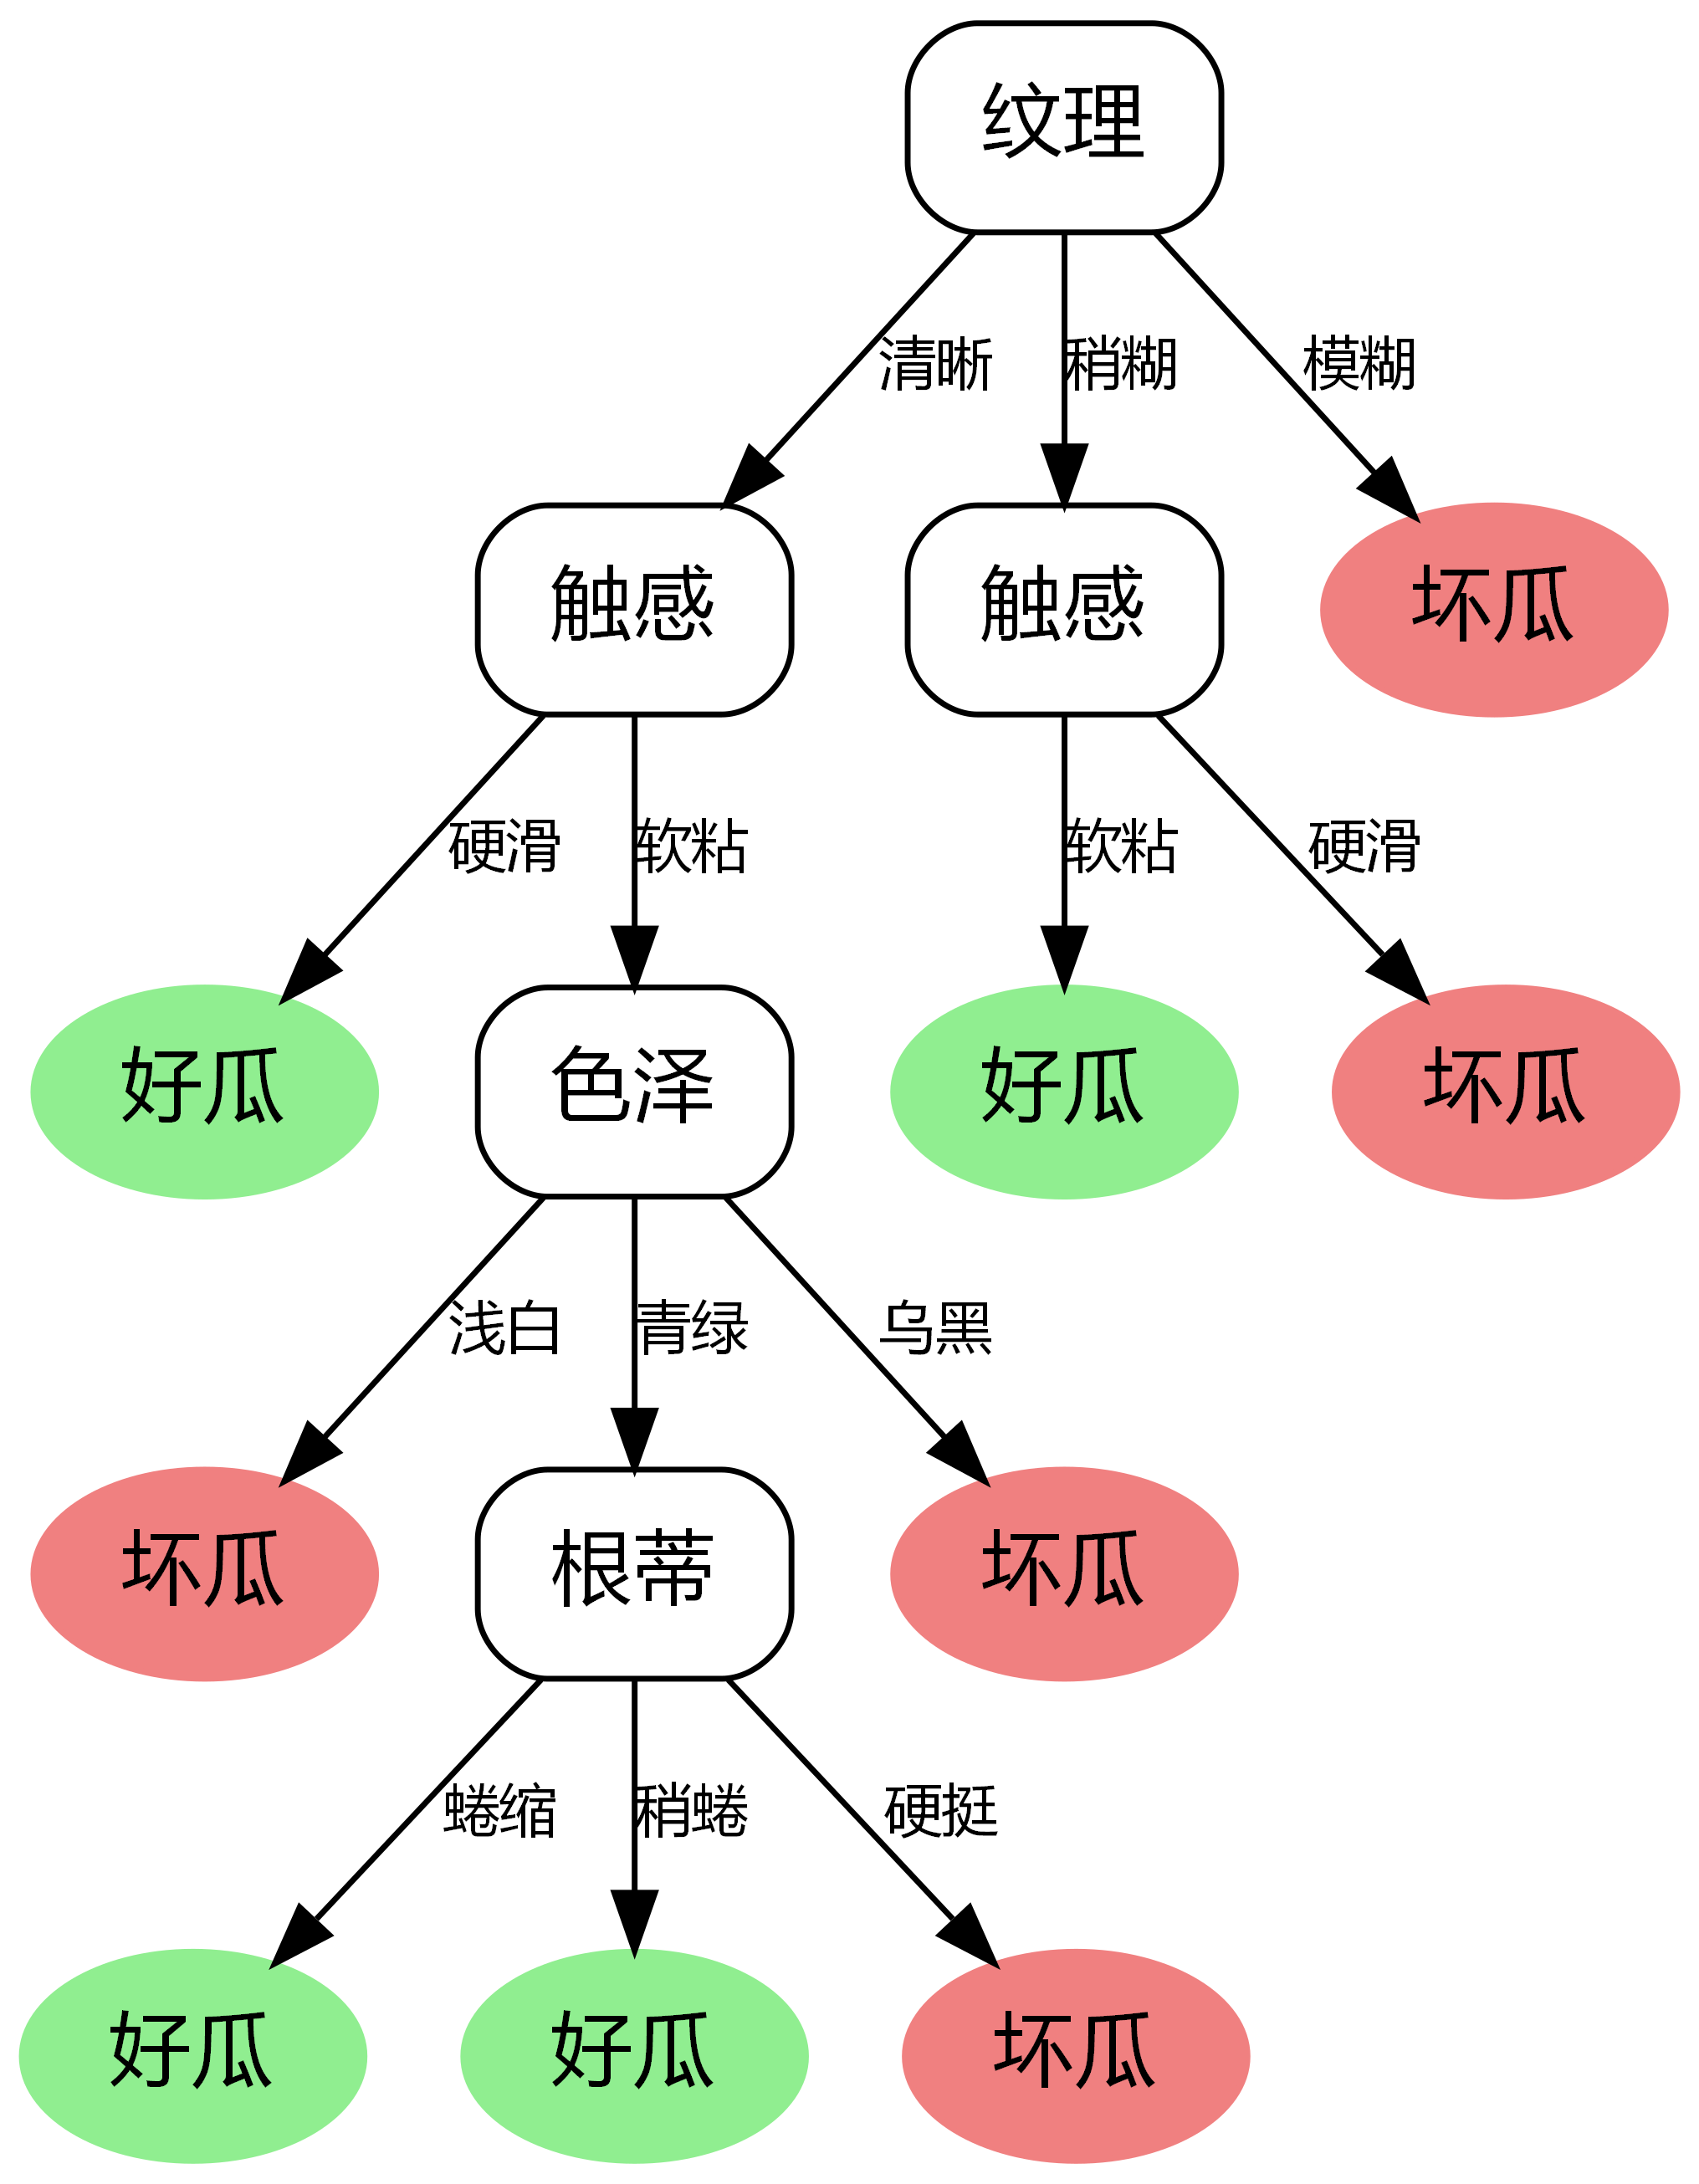
\includegraphics[width=0.5\textwidth]{lab2/fig/decision_tree_C45.png}
    \caption{算法C4.5构建的决策树}
    \end{figure}

    \subsection{算法C4.5程序运行结果截屏}
    \label{fig:C45_result_screenshot}
    \begin{figure}[H]
    \centering
    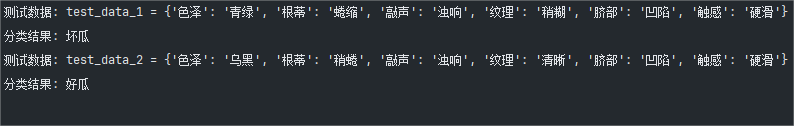
\includegraphics[scale=0.55]{lab2/fig/run_result.png}
    \caption{程序输出的预测结果}
    \end{figure}

\end{document}